\documentclass[9pt,pdf,hyperref={unicode}]{beamer}
\beamertemplatenavigationsymbolsempty

\setbeamertemplate{blocks}[rounded=true, shadow=true]
\setbeamertemplate{footline}[page number]
\usepackage{multicol}

\usefonttheme{serif}

\usepackage[utf8]{inputenc}
\usepackage[english, russian]{babel}
\usepackage{amsmath,mathrsfs,mathtext}
\usepackage{graphicx, epsfig}
\usepackage{caption}
\usepackage{subfig}
\usepackage{amsmath, bm}

\usepackage{comment}

\usepackage{tabularx}

\usepackage{tikz}

\DeclareMathOperator*{\argmin}{arg\,min}
\DeclareMathOperator*{\argmax}{arg\,max}

\makeatletter
\let\@@magyar@captionfix\relax
\makeatother

\usetheme{Warsaw}
\usecolortheme{sidebartab}
\definecolor{beamer@blendedblue}{RGB}{31,96,49}

\setbeamertemplate{enumerate items}[circle]

\setbeamersize{text margin left=1.5em, text margin right=1.5em}

\usepackage{ragged2e}


%----------------------------------------------------------------------------------------------------------
\title[\hbox to 56mm{Смеси экспертов \hfill\insertframenumber\,/\,\inserttotalframenumber}]
{Анализ априорных распределений в задаче смеси экспертов}
\author[А.\,В.~Грабовой]{\large \\Грабовой Андрей Валериевич}
\institute{\large
Московский физико-технический институт}

\date{\footnotesize{МФТИ, г. Долгопрудный}}
%----------------------------------------------------------------------------------------------------------
\begin{document}
%----------------------------------------------------------------------------------------------------------
\begin{frame}
\titlepage
\end{frame}

%----------------------------------------------------------------------------------------------------------
\begin{frame}{Построение ансамбля локальных моделей}
\justifying
\textbf{Цель:} предложить метод построения ансамбля локально аппроксимирующих моделей для поиска окружностей на изображении.

~\\
\textbf{Задачи}

\begin{enumerate}
\justifying
	\item Предложить метод поиска окружности при помощи линейной модели, для поиска нескольких окружностей предложить метод построения смеси локальных аппроксимирующих моделей.
	\item Предложить априорные распределения на параметры локальных моделей.
\end{enumerate}

~\\
\textbf{Исследуемая проблема}
\begin{enumerate}
\justifying
	\item Снижение размерности пространства описаний изображения.
\end{enumerate}

~\\
\textbf{Метод решения}

	В качестве мультимодели предлагается использовать смесь экспертов. Для повышения качества мультимодели предлагается ввести априорные распределения параметров локальных моделей. Вводится \textit{регуляризация} априорных распределений для учета взаимосвязи между априорными распределениями разных локальных моделей смеси.
	
\end{frame}
%----------------------------------------------------------------------------------------------------------
\begin{frame}{Список литературы}
	\begin{enumerate}
	\justifying
		\item \textit{Yuksel Seniha Esen, Wilson Joseph N., Gader Paul D} Twenty Years of Mixture of Experts~// IEEE Transactions on Neural Networks and Learning Systems. 2012. Issues. 23, No 8. pp. 1177--1193.
		\item \textit{A. P. Dempster, N. M. Laird and D. B. Rubin} Maximum Likelihood from Incomplete Data via the EM Algorithm~// Journal of the Royal Statistical Society. Series B (Methodological), Vol. 39, No. 1 pp. 1-38, 1977.
		\item \textit{Bishop C.} Pattern Recognition and Machine Learning.~---~Berlin: Springer, 2006. 758~p.
		\item \textit{I. Matveev} Detection of iris in image by interrelated maxima of brightness gradient projections~// Appl.Comput. Math. 9 (2), 252–257, 2010.
		\item \textit{K. Bowyer, K. Hollingsworth, P. Flynn} A Survey of Iris Biometrics Research: 2008–2010.
		
	\end{enumerate}
\end{frame}

%----------------------------------------------------------------------------------------------------------
\begin{frame}[shrink=5]{Постановка задачи нахождения параметров окружностей}
\justifying
\begin{columns}
\column{0.6\textwidth}
Задано бинарное изображение:
\begin{equation*}
\begin{aligned}
\textbf{M} \in \{0,1\}^{m_1 \times m_2},
\end{aligned}
\end{equation*}
где $1$ --- черная точка, $0$ --- белая точка фона.

По изображению $\textbf{M}$ строится выборка $\textbf{C}$:
\begin{equation*}
\begin{aligned}
\textbf{C} \in  \mathbb{R}^{N \times 2},
\end{aligned}
\end{equation*}
где $N$ --- число черных точек на изображении $\textbf{M}$.
\column{0.36\textwidth}
\begin{center}
	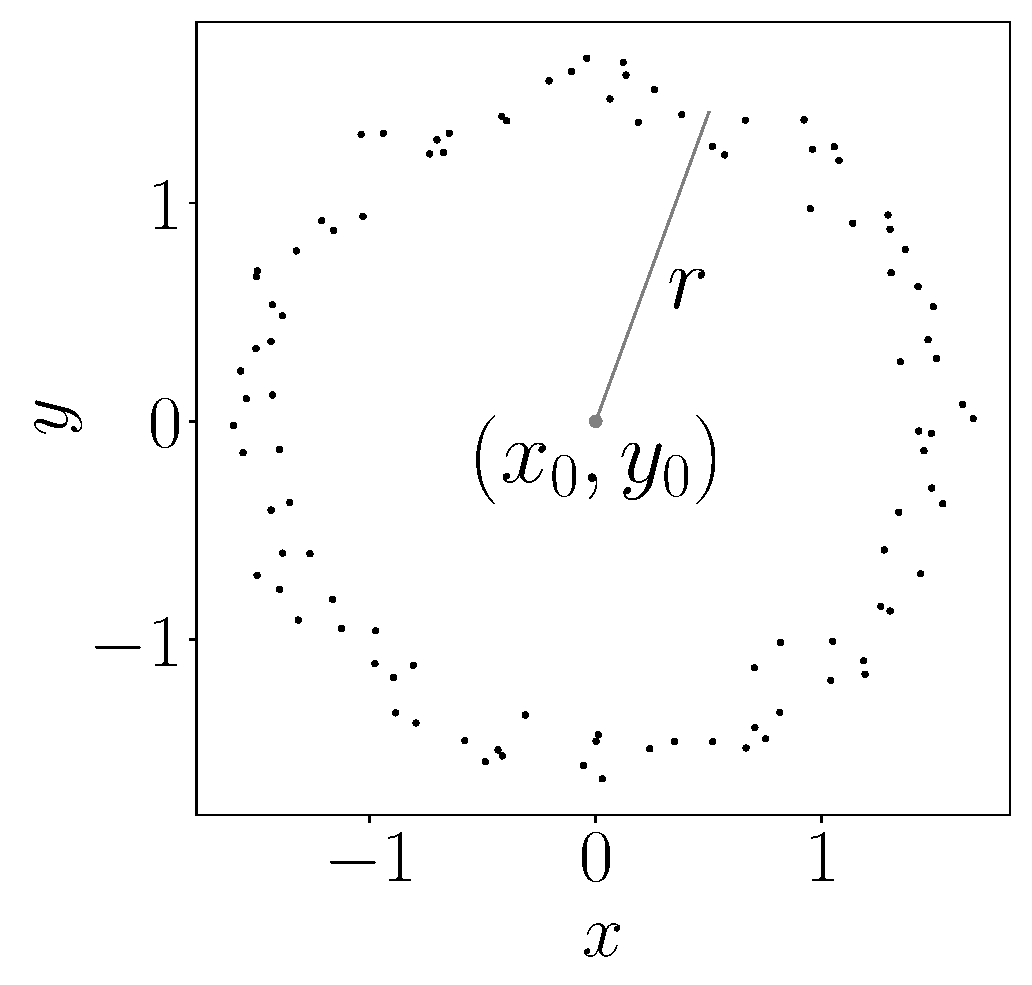
\includegraphics[height=0.4\textheight]{result/slides_statment}
\end{center}
\end{columns}


Пусть $x_0, y_0$~--- центр окружности, которую требуется найти, а $r$ ее радиус.

Точки~$\left(x_i, y_i\right)\in\textbf{C}$ должны удовлетворять уравнению окружности:
\begin{equation*}
\begin{aligned}
\left(x_i - x_0\right)^{2}+\left(y_i-y_0\right)^2 = r^2 \Rightarrow (2x_0)\cdot x_i + (2y_0)\cdot y_i+(r^2-x_0^2-y_0^2)\cdot1 = x_{i}^2 + y_{i}^2.
\end{aligned}
\end{equation*}
Задачу линейной регрессии для нахождения окружности:
\begin{equation*}
\begin{aligned}
\textbf{X}\textbf{w} \approx \textbf{y},  \quad \textbf{X} = \left[\textbf{C}, \textbf{1}\right], \quad \textbf{y} = [x_1^2+y_1^2, x_2^2+y_2^2, \cdots, x_N^2+y_N^2]^{\mathsf{T}},
\end{aligned}
\end{equation*}
где найденые оптимальные параметры линейной регрессии $\textbf{w} = \bigr[w_1, w_2, w_3\bigr]^{\mathsf{T}}$ восстанавливают параметры окружности:
\begin{equation*}
\begin{aligned}
x_0 = \frac{w_1}{2}, \quad y_0 = \frac{w_2}{2}, \quad r = \sqrt[]{w_3+x_{0}^{2}+y_{0}^{2}}.
\end{aligned}
\end{equation*}

\end{frame}
%----------------------------------------------------------------------------------------------------------
\begin{frame}{Универсальная модель--ансамбль: смесь экспертов}
\justifying
Задана выборка:
\begin{equation*}
\begin{aligned}
\textbf{X} \in \mathbb{R}^{N \times n},
\end{aligned}
\end{equation*}
где~$N$~---~число объектов в выборке, а~$n$~---~размерность признакового пространства.


\begin{definition}
Смесь экспертов~---~мультимодель, определяющая правдоподобие веса $\pi_k$ каждой локальной модели $\textbf{f}_k$ на признаковом описании объекта $\textbf{x}$.
\begin{equation*}
\begin{aligned}
\hat{\mathbf{f}} = \sum_{k=1}^{K}\pi_{k}\mathbf{f}_k, \qquad \pi_{k}\left(\mathbf{x}, \mathbf{V}\right):\mathbb{R}^{n\times \left|\mathbf{V}\right|} \to [0, 1], \qquad \sum_{k=1}^{K}\pi_{k}\left(\mathbf{x}, \mathbf{V}\right) = 1,
\end{aligned}
\end{equation*}
где~$\hat{\mathbf{f}}$~---~мультимодель, а $\mathbf{f}_k$ является локальной моделью, $\pi_k$~---~шлюзовая функция, $\mathbf{w}_k$~---~параметры $k$-й локальной модели, $\mathbf{V}$~---~параметры шлюзовой функции.
\end{definition}

В качестве локальных моделей~$\mathbf{f}_k$ и шлюзовой функции~$\bm{\pi}$ рассматриваются следующие функции:
\begin{equation*}
\begin{aligned}
\mathbf{f}_k\left(\textbf{x}\right) = \textbf{w}_k^{\mathsf{T}}\textbf{x}, \quad
\bm{\pi}\left(\mathbf{x}, \mathbf{V}\right) = \text{softmax}\bigr(\mathbf{V}_{1}^{\mathsf{T}}\bm{\sigma}\bigr(\mathbf{V}_2^{\mathsf{T}}\mathbf{x}\bigr)\bigr),
\end{aligned}
\end{equation*}
где $\mathbf{V} = \bigr\{\mathbf{V}_1, \mathbf{V}_2\bigr\}$~---~параметры шлюзовой функции.


\end{frame}
%----------------------------------------------------------------------------------------------------------
\begin{frame}{Оптимизация параметров}
\justifying
Параметры локальных моделей оптимизируются согласно принципу максимального правдоподобия модели:
\begin{equation*}
\begin{aligned}
p\bigr(\mathbf{y}, \mathbf{W}|\mathbf{X}, \mathbf{V}\bigr) = \prod_{k=1}^{K}p^{k}\bigr(\mathbf{w}_k\bigr)\prod_{i=1}^{N}\left(\sum_{k=1}^{K}\pi_{k}p_{k}\bigr(y_i|\mathbf{w}_k, \mathbf{x}_i\bigr)\right),
\end{aligned}
\end{equation*}
где $\mathbf{W} = \bigr[\mathbf{w}_1, \mathbf{w}_2, \cdots, \mathbf{w}_K\bigr]^{\mathsf{T}}.$

Задача оптимизации параметров локальных моделей и параметров смеси:
\begin{equation*}
\begin{aligned}
\hat{\mathbf{W}}, \hat{\mathbf{V}} = \arg\max_{\mathbf{W}, \mathbf{V}} p\bigr(\mathbf{y}, \mathbf{W}|\mathbf{X}, \mathbf{V}\bigr).
\end{aligned}
\end{equation*}

Рассматривается вероятностная постановка задачи:
\begin{enumerate}
	\item[1)] правдоподобие выборки $p_{k}\left(y_{i}|\mathbf{w}_{k}, \mathbf{x}_{i}\right) = \mathcal{N}\left(y_{i}|\mathbf{w}_{k}^{\mathsf{T}}\mathbf{x}_{i}, \beta^{-1}\right),$ где $\beta$ уровень шума,
	\item[2)] априорное распределение параметров $p^{k}\left(\mathbf{w}_{k}\right) = \mathcal{N}\left(\mathbf{w}_{k}|\mathbf{w}^{0}_{k}, \mathbf{A}_{k}\right),$ где $\mathbf{w}^{0}_{k}$~---~вектор размера $n\times1,$ $\mathbf{A}_{k}$~---~ковариационная матрица параметров,
	\item[3)] регуляризация априорного распределения $p\left(\bm{\varepsilon}_{k,k'}|\bm{\alpha}\right) = \mathcal{N}\left(\bm{\varepsilon}_{k,k'}|\mathbf{0},  \bm{\Xi}\right),$ где~$\bm{\Xi}$~---~ковариационная матрица общего вида, $\bm{\varepsilon}_{k,k'} = \mathbf{w}_{k}^{0}-\mathbf{w}_{k'}^{0}.$
\end{enumerate}

\end{frame}
%----------------------------------------------------------------------------------------------------------
\begin{frame}{EM--алгоритм для решения задачи смеси экспертов}
\justifying
Правдоподобие модели включает правдоподобие выборки, априорное распределение параметров, а также их регуляризацию
\begin{equation*}
\begin{aligned}
p\bigr(\mathbf{y}, \mathbf{W}|\mathbf{X}, \mathbf{V}, \textbf{A}, \textbf{W}^{0}, \bm{\Xi}, \beta\bigr) = &\prod_{k,k'=1}^{K}\mathcal{N}\left(\bm{\varepsilon}_{k,k'}|\mathbf{0},  \bm{\Xi}\right)\cdot\\
&\cdot\prod_{k=1}^{K}\mathcal{N}\left(\mathbf{w}_{k}|\mathbf{w}^{0}_{k}, \mathbf{A}_{k}\right)\prod_{i=1}^{N}\left(\sum_{k=1}^{K}\pi_{k}\mathcal{N}\left(y_{i}|\mathbf{w}_{k}^{\mathsf{T}}\mathbf{x}_{i}, \beta^{-1}\right)\right),
\end{aligned}
\end{equation*}
где~$\mathbf{A} = \bigr\{\mathbf{A}_1, \cdots, \mathbf{A}_K\bigr\}.$
Введем скрытые переменные $\textbf{Z} = [z_{ik}],$ где $~z_{ik} = 1$ тогда и только тогда, когда $k_i=k$:
\begin{equation*}
\begin{aligned}
\log p\bigr(\mathbf{y}, \mathbf{Z}, \mathbf{W}&|\mathbf{X}, \mathbf{V}, \textbf{A}, \textbf{W}^{0},  \bm{\Xi}, \beta\bigr) =\\
&= \sum_{i=1}^{N}\sum_{k=1}^{K}z_{ik}\left[\log\pi_k\left(\textbf{x}_i, \textbf{V}\right) - \frac{\beta}{2}\left(y_{i} - \textbf{w}_{k}^{\mathsf{T}}\textbf{x}_{i}\right)^{2} + \frac{1}{2}\log\frac{\beta}{2\pi}\right] +\\
&+ \sum_{k=1}^{K}\left[-\frac{1}{2}\left(\textbf{w}_{k} - \textbf{w}_{k}^{0}\right)^{\mathsf{T}}\textbf{A}_{k}^{-1}\left(\textbf{w}_{k} - \textbf{w}_{k}^{0}\right) + \frac{1}{2}\log\det\textbf{A}^{-1}_{k} - \frac{n}{2}\log2\pi\right]+\\
&+ \sum_{k=1}^{K}\sum_{k'=1}^{K}\left[-\frac{1}{2}\left(\textbf{w}_{k}^{0}-\textbf{w}_{k'}^{0}\right)^{\mathsf{T}}\hat{\bm{\alpha}}^{-1}\left(\textbf{w}_{k}^{0}-\textbf{w}_{k'}^{0}\right) +\frac{1}{2}\log\det \bm{\Xi} -\frac{n}{2}\log{2\pi}\right].
\end{aligned}
\end{equation*}

\end{frame}
%----------------------------------------------------------------------------------------------------------
\begin{frame}{EM--алгоритм для решения задачи смеси экспертов}
\justifying
Задача оптимизации параметров локальных моделей и параметров смеси принимает следующий вид:
\begin{equation*}
\begin{aligned}
\mathbf{W}, \mathbf{Z}, \mathbf{V}, \mathbf{W}^0, \textbf{A},  \beta = \arg\max_{\mathbf{W}, \mathbf{Z}, \mathbf{V}, \mathbf{W}^0, \textbf{A}, \beta} \log p\bigr(\mathbf{y}, \mathbf{Z}, \mathbf{W}&|\mathbf{X}, \mathbf{V}, \textbf{A}, \textbf{W}^{0}, \bm{\Xi}, \beta\bigr).
\end{aligned}
\end{equation*}

Для оптимизации используется вариационный ЕМ--алгоритм с аппроксимацией среднего поля~$q\left(\textbf{Z}, \textbf{W}\right) = q\left(\textbf{Z}\right)q\left(\textbf{W}\right)$.

Е и М шаги алгоритма имеют следующий вид:
	\begin{enumerate}
		\item Е--шаг: 
			\begin{equation*}
				\begin{aligned}
					\log q\left(\textbf{Z}^{s}\right) &\propto \mathsf{E}_{q/\textbf{Z}}\log p\bigr(\mathbf{y}, \textbf{Z},\mathbf{W}|\mathbf{X}, \mathbf{V}^{s-1}, \textbf{A}^{s-1}, \textbf{W}^{0, s-1}, \bm{\Xi}, \beta^{s-1}\bigr),\\
					\log q\left(\textbf{W}^{s}\right) &\propto \mathsf{E}_{q/\textbf{W}}\log p\bigr(\mathbf{y}, \textbf{Z},\mathbf{W}|\mathbf{X}, \mathbf{V}^{s-1}, \textbf{A}^{s-1}, \textbf{W}^{0, s-1}, \bm{\Xi}, \beta^{s-1}\bigr),
				\end{aligned}
			\end{equation*}
		\item М--шаг: 
			\begin{equation*}
				\begin{aligned}
					\textbf{W}^{0, s}, \textbf{A}^{s}, \textbf{V}^{s}, \beta^{s} = \arg\max_{\textbf{W}^{0}, \textbf{A}, \textbf{V}, \beta} \mathsf{E}_{q^{s}}\log p\bigr(\mathbf{y}, \textbf{Z},\mathbf{W}|\mathbf{X}, \mathbf{V}, \textbf{A}, \textbf{W}^{0}, \bm{\Xi}, \beta\bigr),
				\end{aligned}
			\end{equation*}
	\end{enumerate}
	где~$s$~--- номер итерации.
\end{frame}
%----------------------------------------------------------------------------------------------------------
\begin{frame}{EM--алгоритм для решения задачи смеси экспертов}
\justifying
Итерационные формулы ЕМ--алгоритма:
	\begin{enumerate}
		\item Е--шаг: 
			\begin{equation*}
				\begin{aligned}
					&p\left(z_{ik} = 1\right) = \frac{\exp\left(\log\pi_{k}\left(\textbf{x}_{i}, \textbf{V}\right) - \frac{\beta}{2}\left(\textbf{x}_{i}^{\mathsf{T}}\mathsf{E}\textbf{w}_{k}\textbf{w}_{k}^{\mathsf{T}}\textbf{x}_{i} - \textbf{x}_{i}^{\mathsf{T}}\mathsf{E}\textbf{w}_{k}\right)\right)}{\sum_{k'=1}^{K}\exp\left(\log\pi_{k'}\left(\textbf{x}_{i}, \textbf{V}\right) - \frac{\beta}{2}\left(\textbf{x}_{i}^{\mathsf{T}}\mathsf{E}\textbf{w}_{k'}\textbf{w}_{k'}^{\mathsf{T}}\textbf{x}_{i} - \textbf{x}_{i}^{\mathsf{T}}\mathsf{E}\textbf{w}_{k'}\right) \right)},\\
					&q(\textbf{w}_k) = \mathcal{N}(\textbf{w}_k|\textbf{m}_k, \textbf{B}_k),\\
					&\mathbf{m}_{k} = \mathbf{B}_{k}\left(\mathbf{A}_{k}^{-1}\mathbf{w}_{k}^{0}+\beta\sum_{i=1}^{N}\mathbf{x}_{i}y_{i}\mathsf{E}z_{ik}\right), \quad
					\mathbf{B}_{k} = \left(\mathbf{A}_{k}^{-1}+\beta\sum_{i=1}^{N}\mathbf{x}_{i}\mathbf{x}_{i}^{\mathsf{T}}\mathsf{E}z_{ik}\right)^{-1} .
				\end{aligned}
			\end{equation*}
		\item М--шаг: 
			\begin{equation*}
				\begin{aligned}
					&\textbf{A}_{k} = \mathsf{E}\textbf{w}_{k}\textbf{w}_{k}^{\mathsf{T}} - \textbf{w}_{k}^{0}\mathsf{E}\textbf{w}_{k}^{\mathsf{T}} - \mathsf{E}\textbf{w}_{k}\textbf{w}_{k}^{0\mathsf{T}} + \textbf{w}_{k}^{0}\textbf{w}_{k}^{0\mathsf{T}}, \\
					 &\frac{1}{\beta}=\frac{1}{N}\sum_{i=1}^{N}\sum_{k=1}^{K}\left[y_{i}^{2}-2y_{i}\textbf{x}_{i}^{\mathsf{T}}\mathsf{E}\textbf{w}_{k} + \textbf{x}_{i}^{\mathsf{T}}\mathsf{E}\textbf{w}_{k}\textbf{w}_{k}^{\mathsf{T}}\textbf{x}_{i}\right]\mathsf{E}z_{ik},\\
					&\textbf{w}_{k}^{0} =\left[\textbf{A}_{k}^{-1}+\left(K-1\right)\bm{\Xi}\right]^{-1}\left(\textbf{A}^{-1}_{k}\mathsf{E}\textbf{w}_{k}+\bm{\Xi}\sum_{k'=1,~k'\not=k}^{K}\textbf{w}_{k'}^{0}\right),\\
					&\textbf{V}= \arg\max_{\textbf{V}} \mathsf{E}_{q^{s}}\log p\bigr(\mathbf{y}, \textbf{Z},\mathbf{W}|\mathbf{X}, \mathbf{V}, \textbf{A}, \textbf{W}^{0}, \bm{\Xi}, \beta\bigr).
				\end{aligned}
			\end{equation*}
	\end{enumerate}
\end{frame}
%----------------------------------------------------------------------------------------------------------
\begin{frame}{Вычислительный эксперимент}
\justifying
Вычислительный эксперимент делится на следующие этапы:
\begin{enumerate}
	\item Анализ синтетических данных с разным типом шума в изображении;
	\item Анализ изменения параметров локальных моделей во время обучения;
	\item Анализ мультимоделей в зависимости от уровня шума в изображении;
	\item Анализ качества модели на реальных данные.
\end{enumerate}

Гиперпараметры заданы следующим образом:
\begin{enumerate}
	\item Априорные распределения на параметры локальных моделей в эксперименте задано следующим образом:
\begin{equation*}
\begin{aligned}
p^{1}\left(\textbf{w}_1\right)\sim\mathcal{N}\left(\textbf{w}^{0}_{1}, \textbf{I}\right), \quad p^{2}\left(\textbf{w}_2\right)\sim\mathcal{N}\left(\textbf{w}^{0}_{2}, \textbf{I}\right),
\end{aligned}
\end{equation*}
где $\textbf{w}^{0}_1 = [0, 0, 0.1],\ \textbf{w}^{0}_2 = [0, 0, 2]$.

	\item Параметр регуляризации:
\begin{equation*}
\begin{aligned}
\bm{\Xi} = \begin{bmatrix}
0.01& 0 & 0\\
0& 0.01 & 0\\
0& 0 & 1\\
\end{bmatrix},
\end{aligned}
\end{equation*}
что указывает на концентричность окружностей.
\end{enumerate}

\end{frame}
%----------------------------------------------------------------------------------------------------------
\begin{frame}{Синтетические данные с разным типом шума в изображении}
\justifying
\begin{center}
	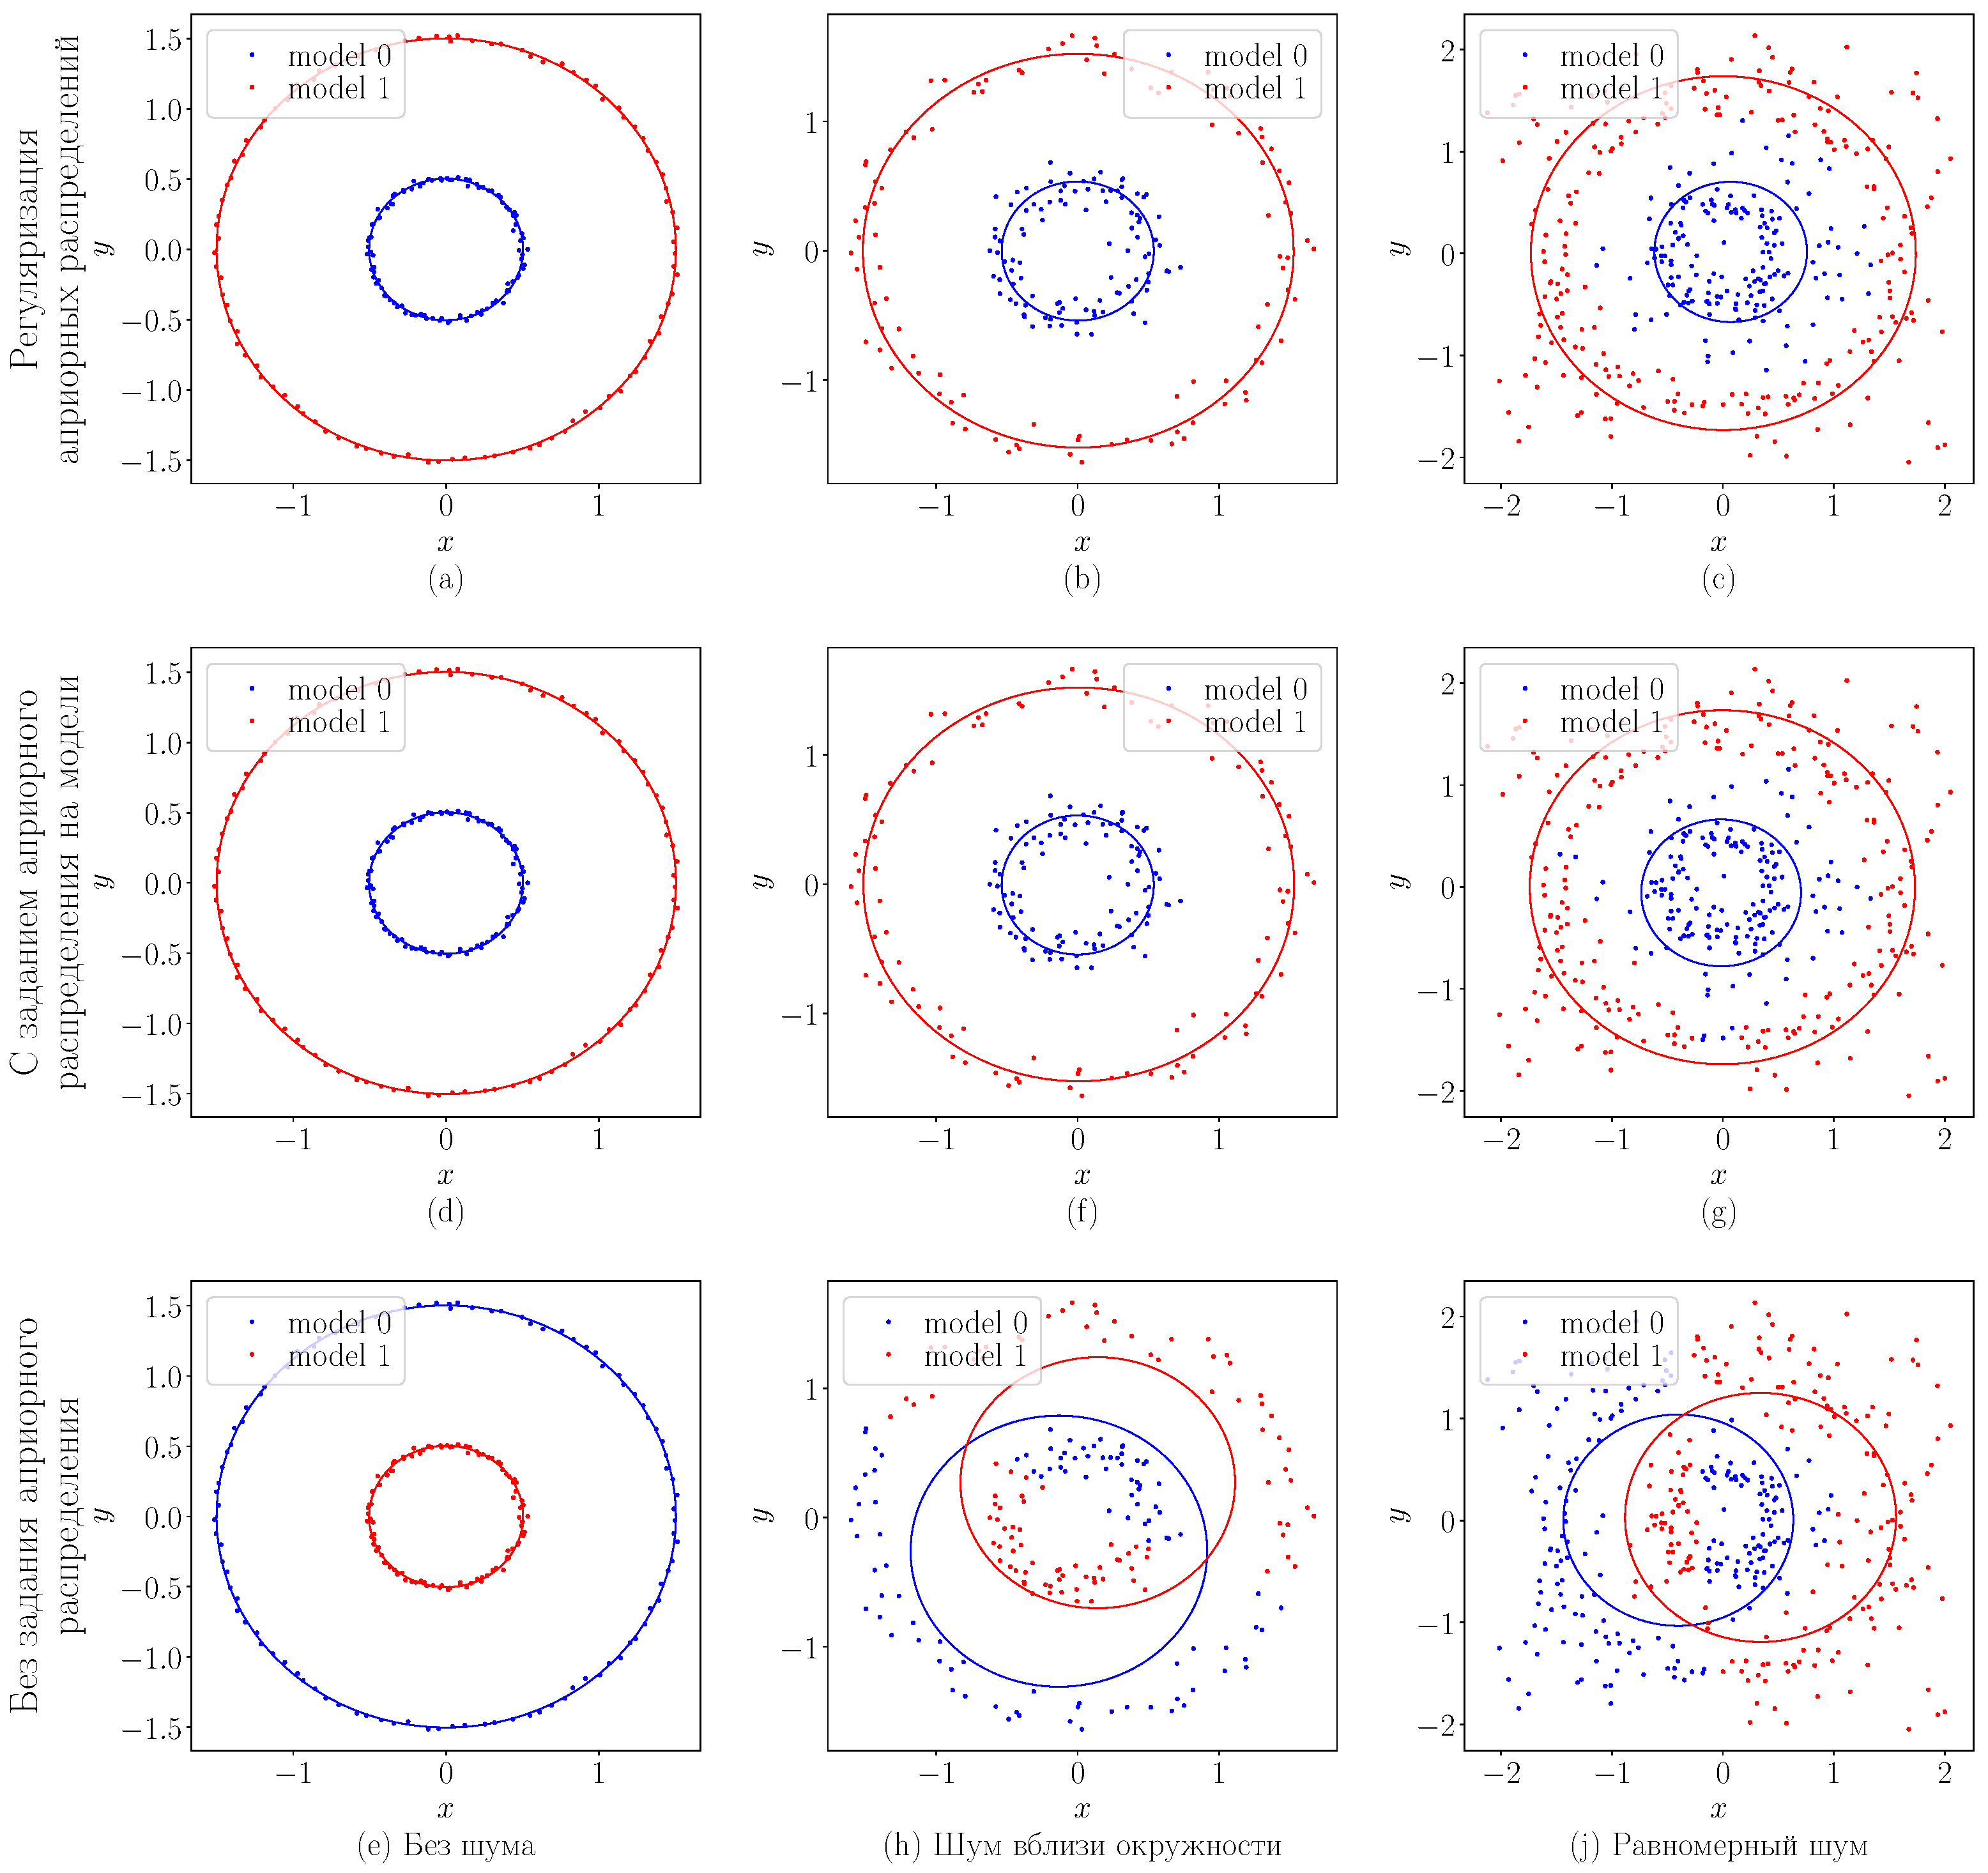
\includegraphics[height=0.9\textheight]{result/experiment_synthetic}
\end{center}

\end{frame}
%----------------------------------------------------------------------------------------------------------
\begin{frame}{Параметры локальных моделей в процессе обучения}
\justifying
\begin{center}
	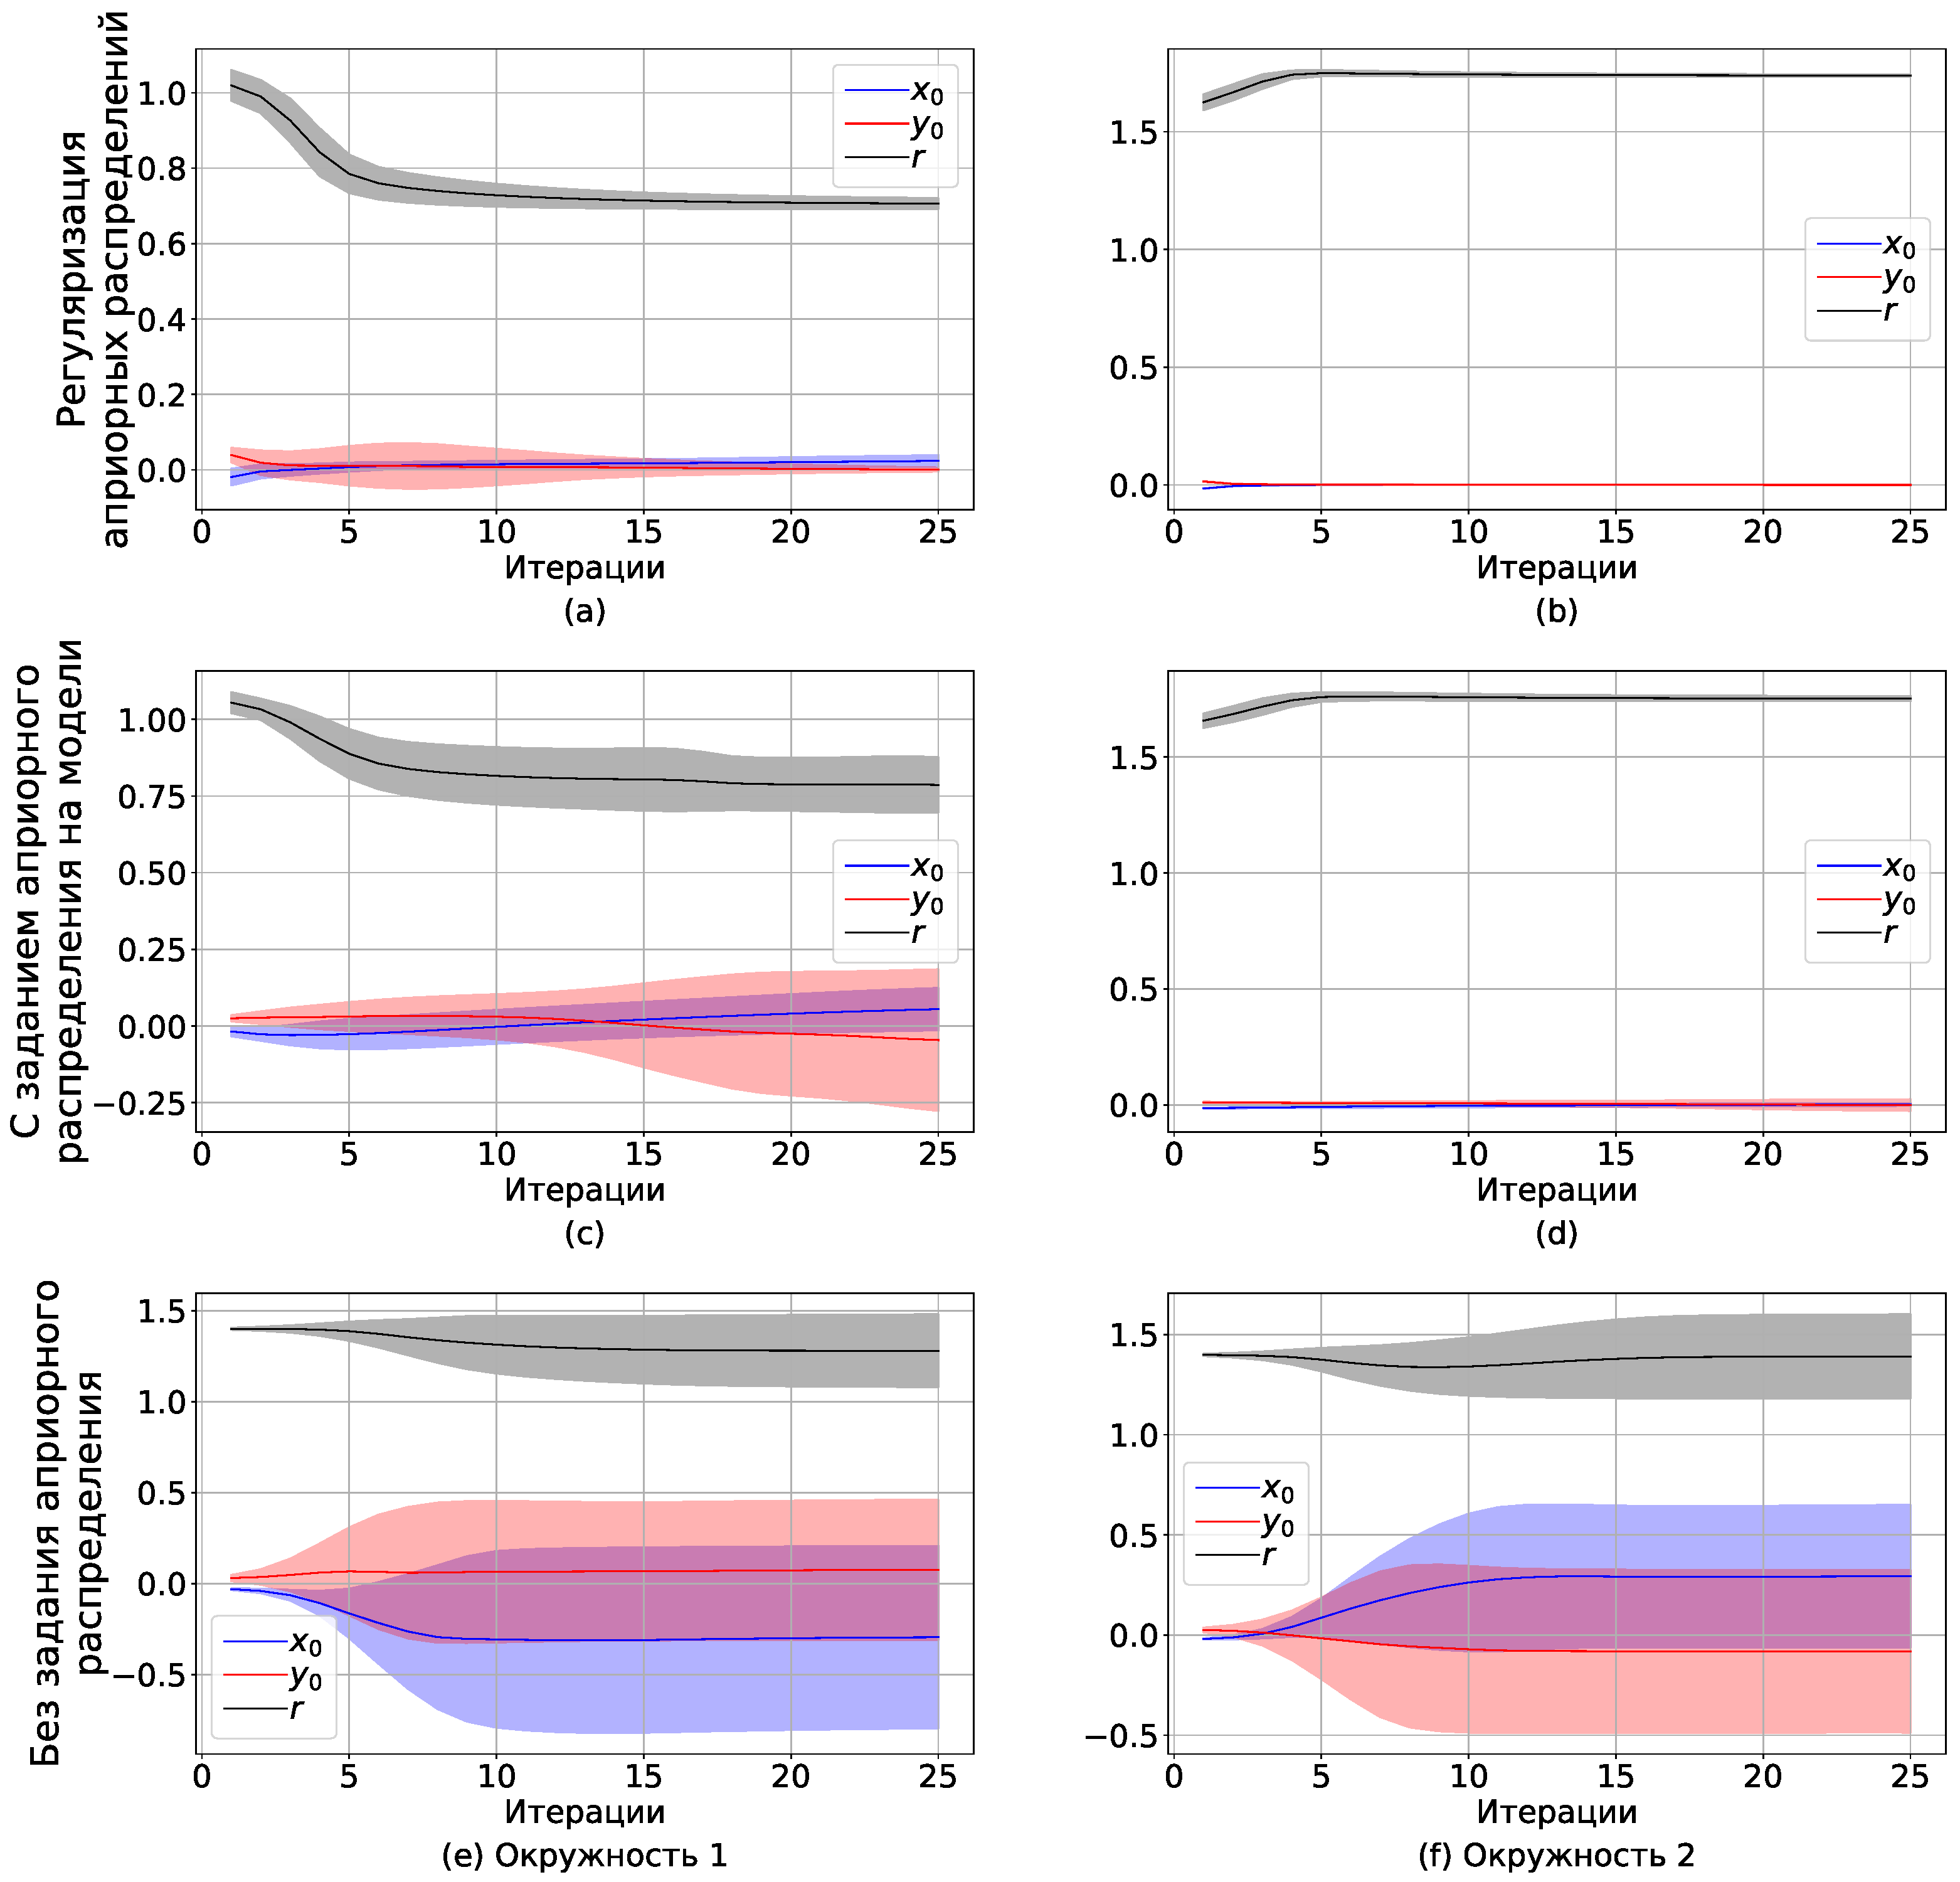
\includegraphics[height=0.9\textheight]{result/experiment_synthetic_param_progress}
\end{center}

\end{frame}
%----------------------------------------------------------------------------------------------------------
\begin{frame}{Обучения на синтетических данных}
\justifying
Регуляризация априорных распределений
\begin{center}
	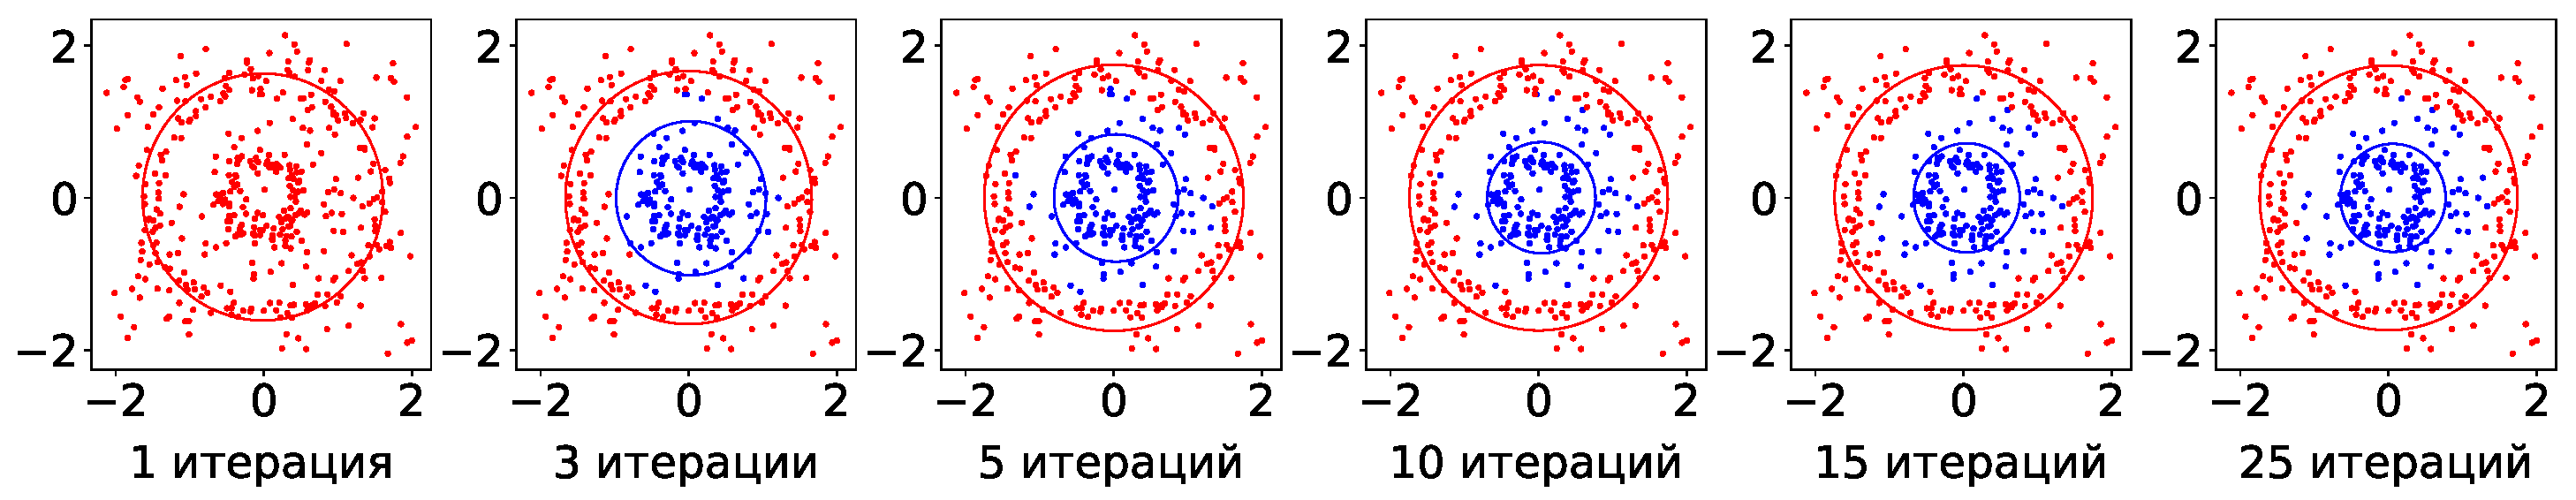
\includegraphics[width=0.95\textwidth]{result/experiment_synt_regular_progress}
\end{center}
С заданием априорного распределения на модели
\begin{center}
	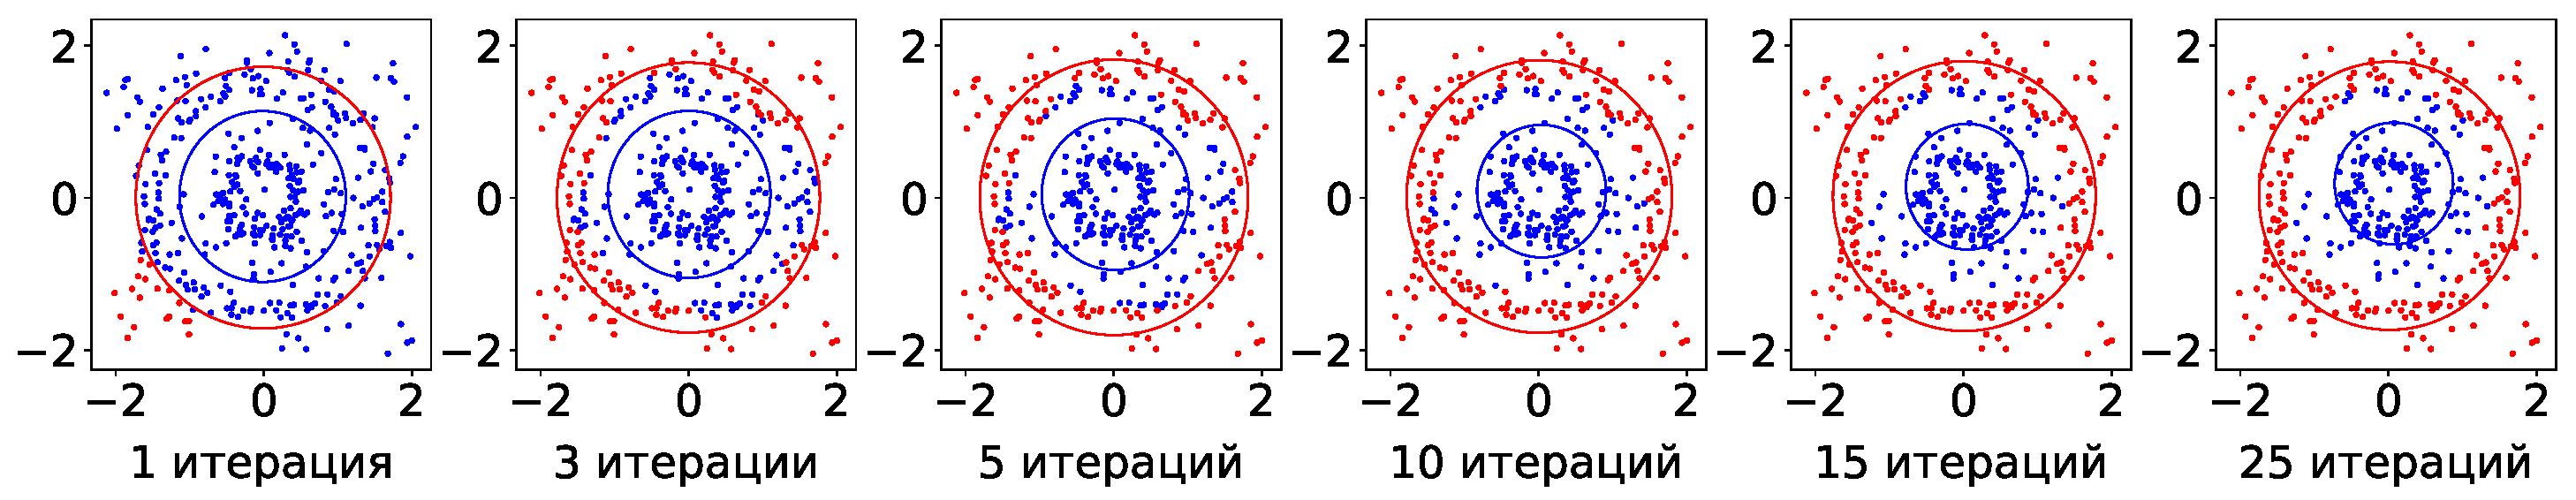
\includegraphics[width=0.95\textwidth]{result/experiment_synt_prior_progress}
\end{center}
Без задания априорного распределения
\begin{center}
	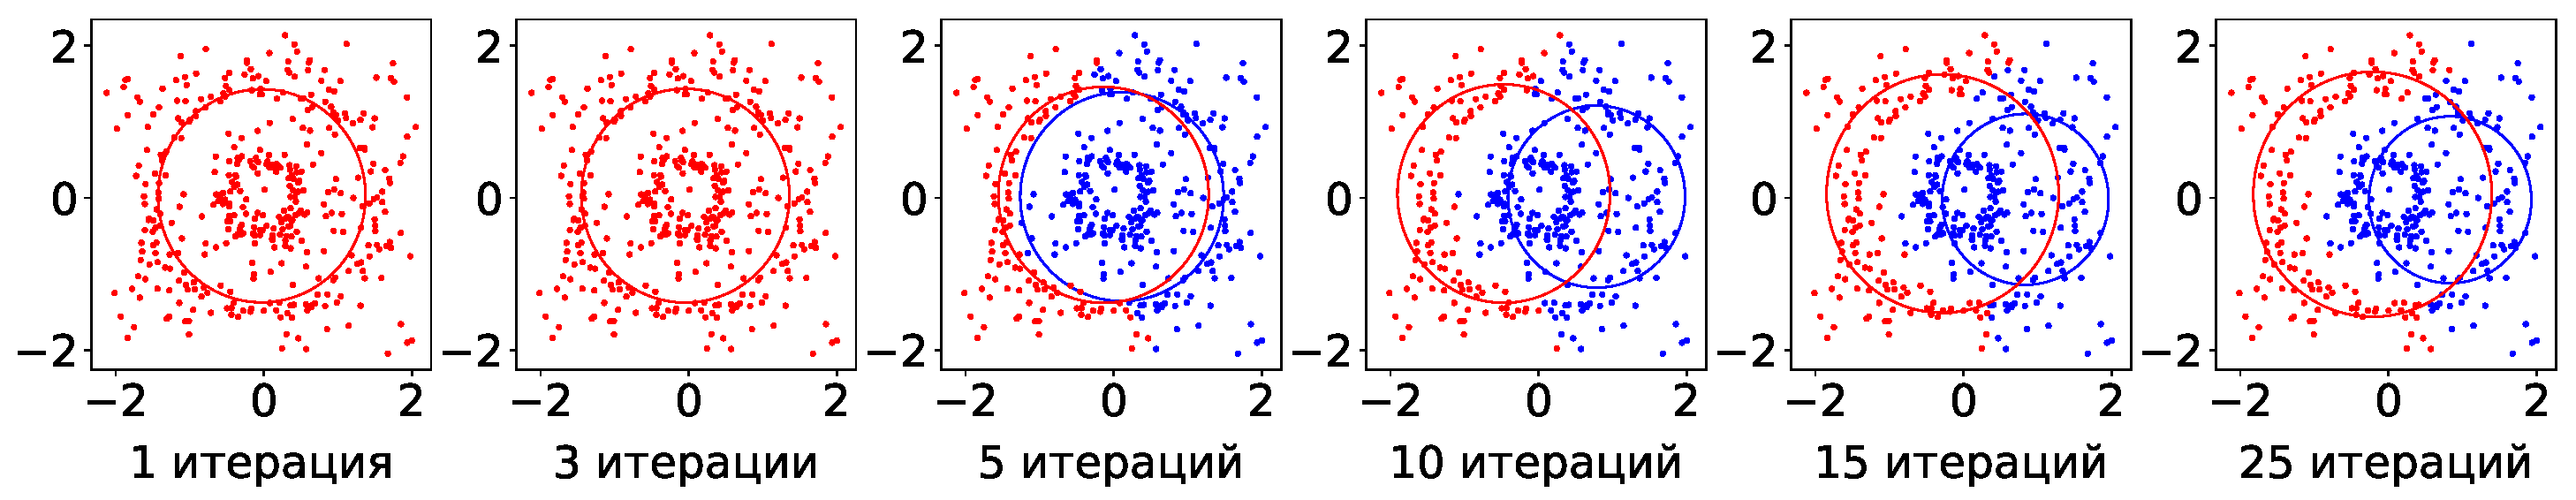
\includegraphics[width=0.95\textwidth]{result/experiment_synt_not_prior_progress}
\end{center}
\end{frame}
%----------------------------------------------------------------------------------------------------------
\begin{frame}{Анализ мультимоделей в зависимости от уровня шума}
\justifying
\begin{center}
	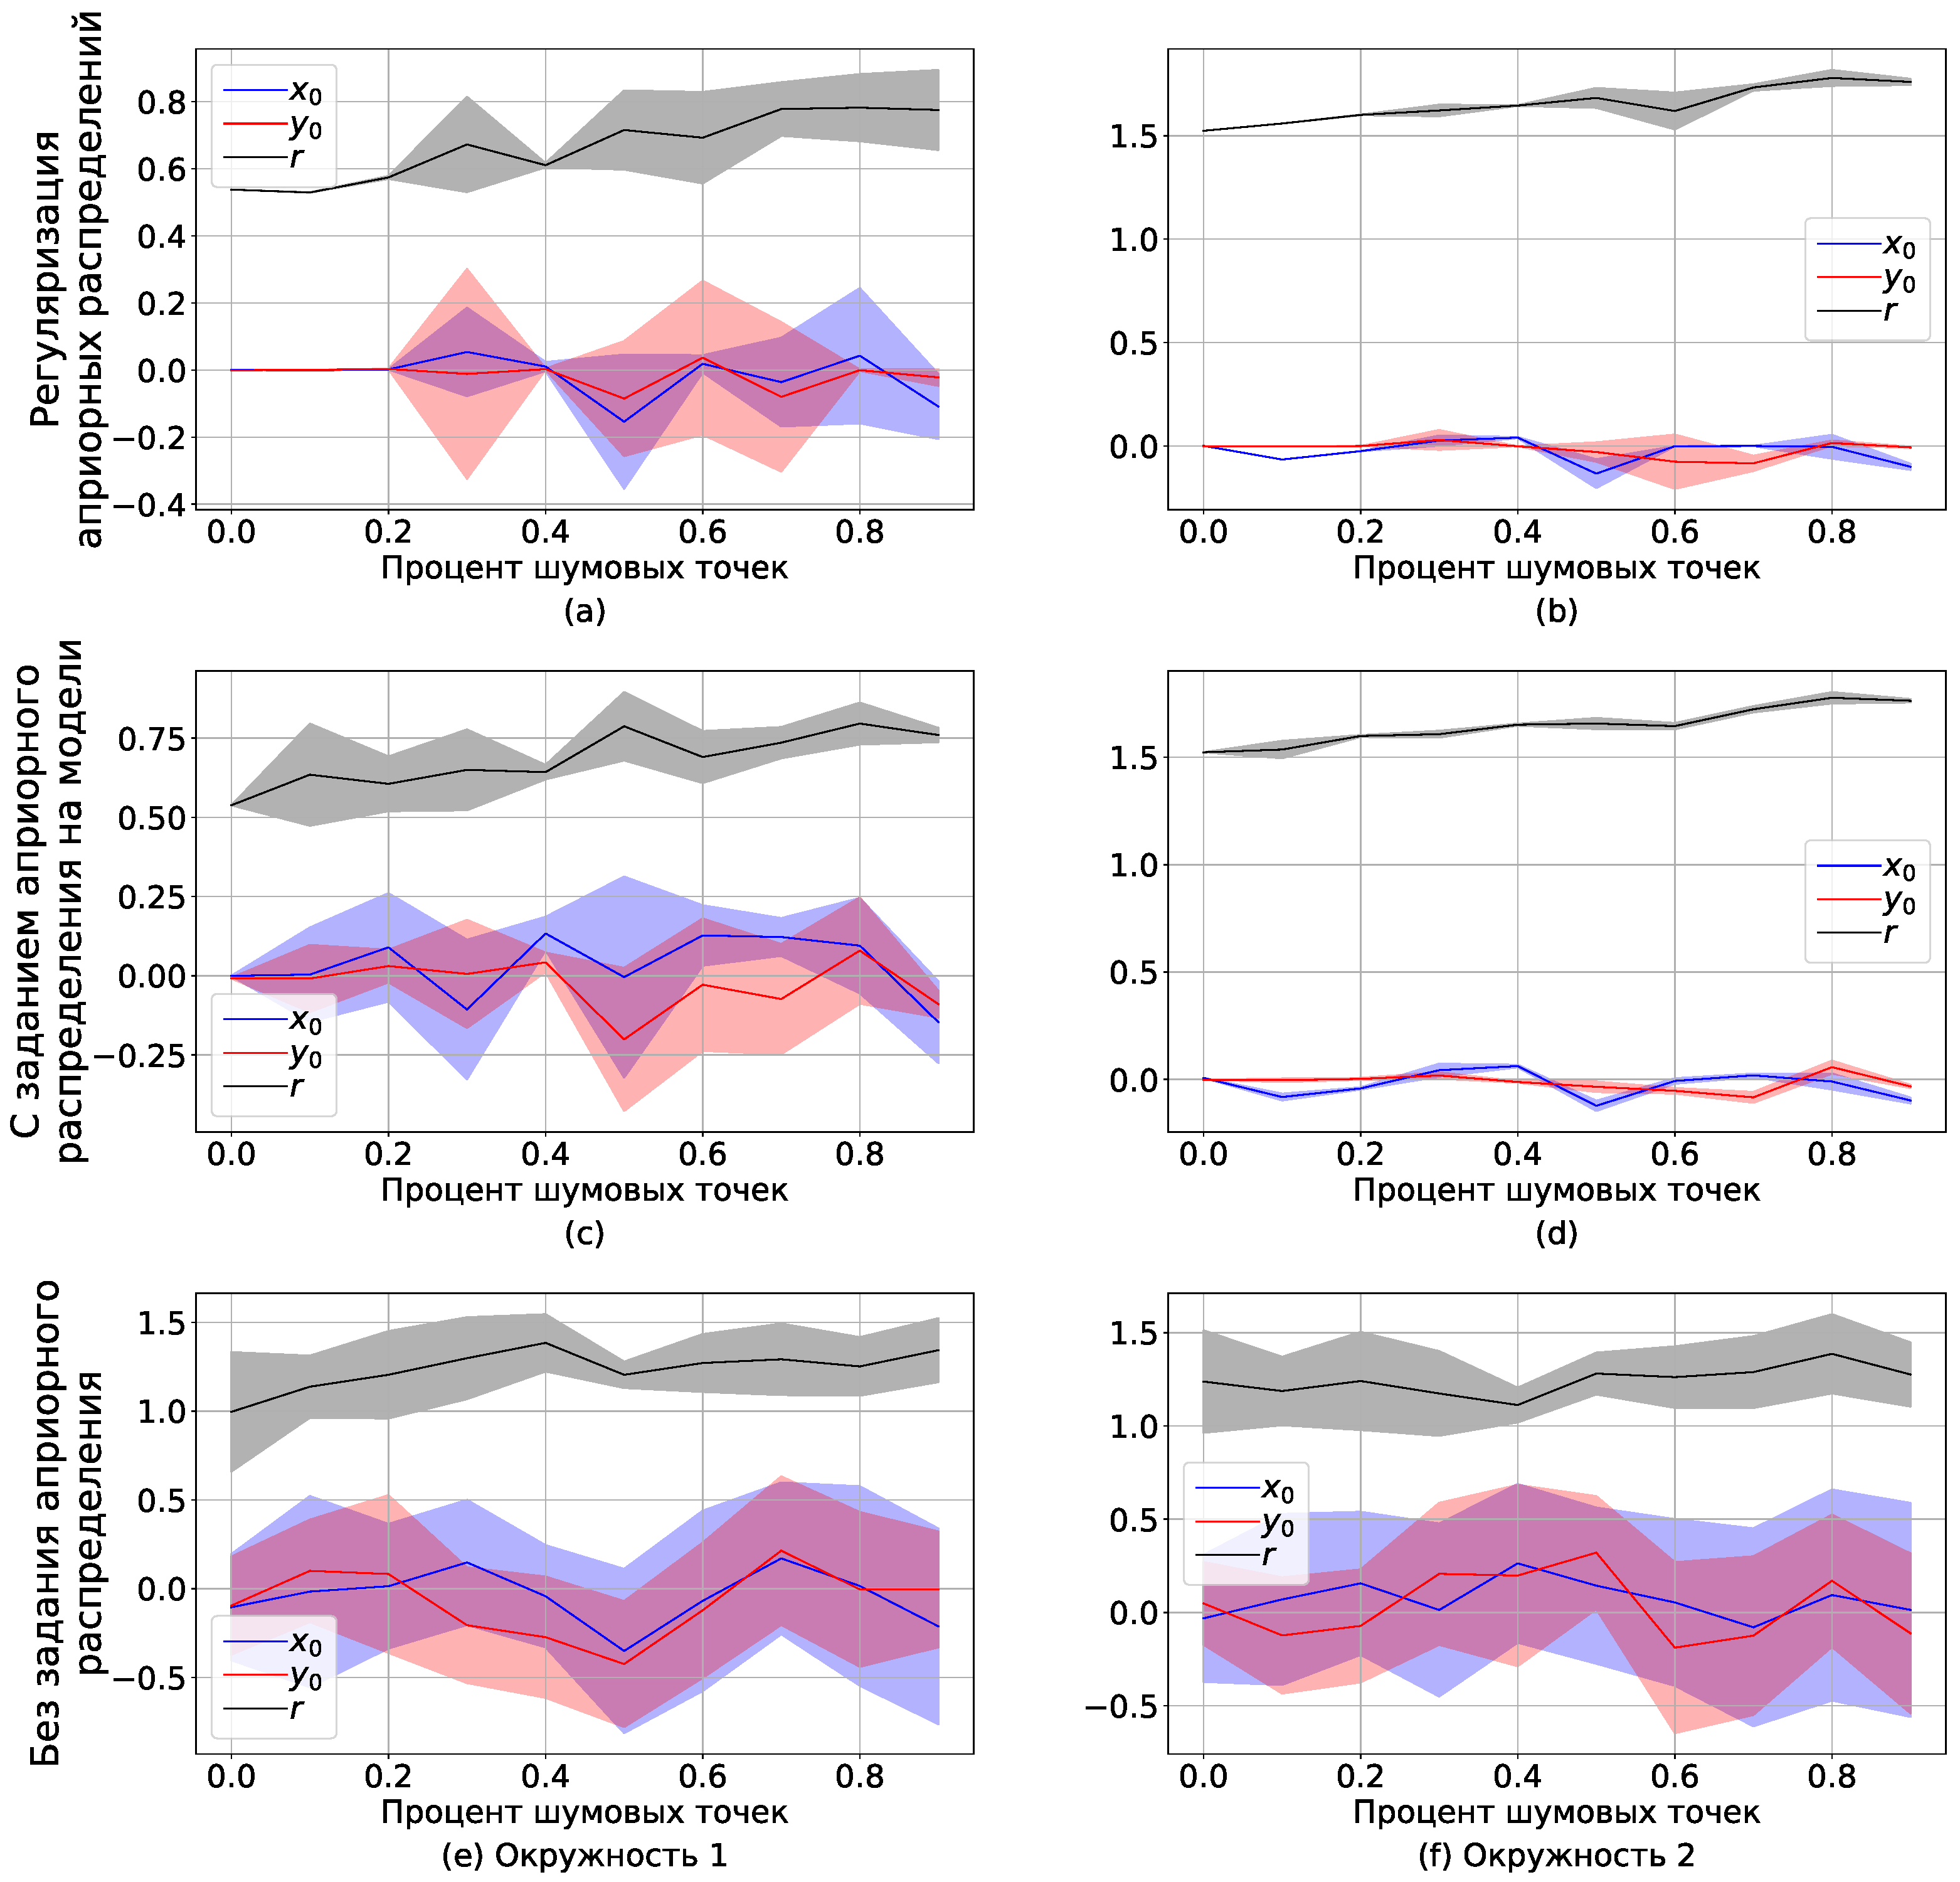
\includegraphics[height=0.9\textheight]{result/experiment_synthetic_param_progress_noise}
\end{center}

\end{frame}
%----------------------------------------------------------------------------------------------------------
\begin{frame}{Результаты на реальных данных}
\justifying
\begin{center}
	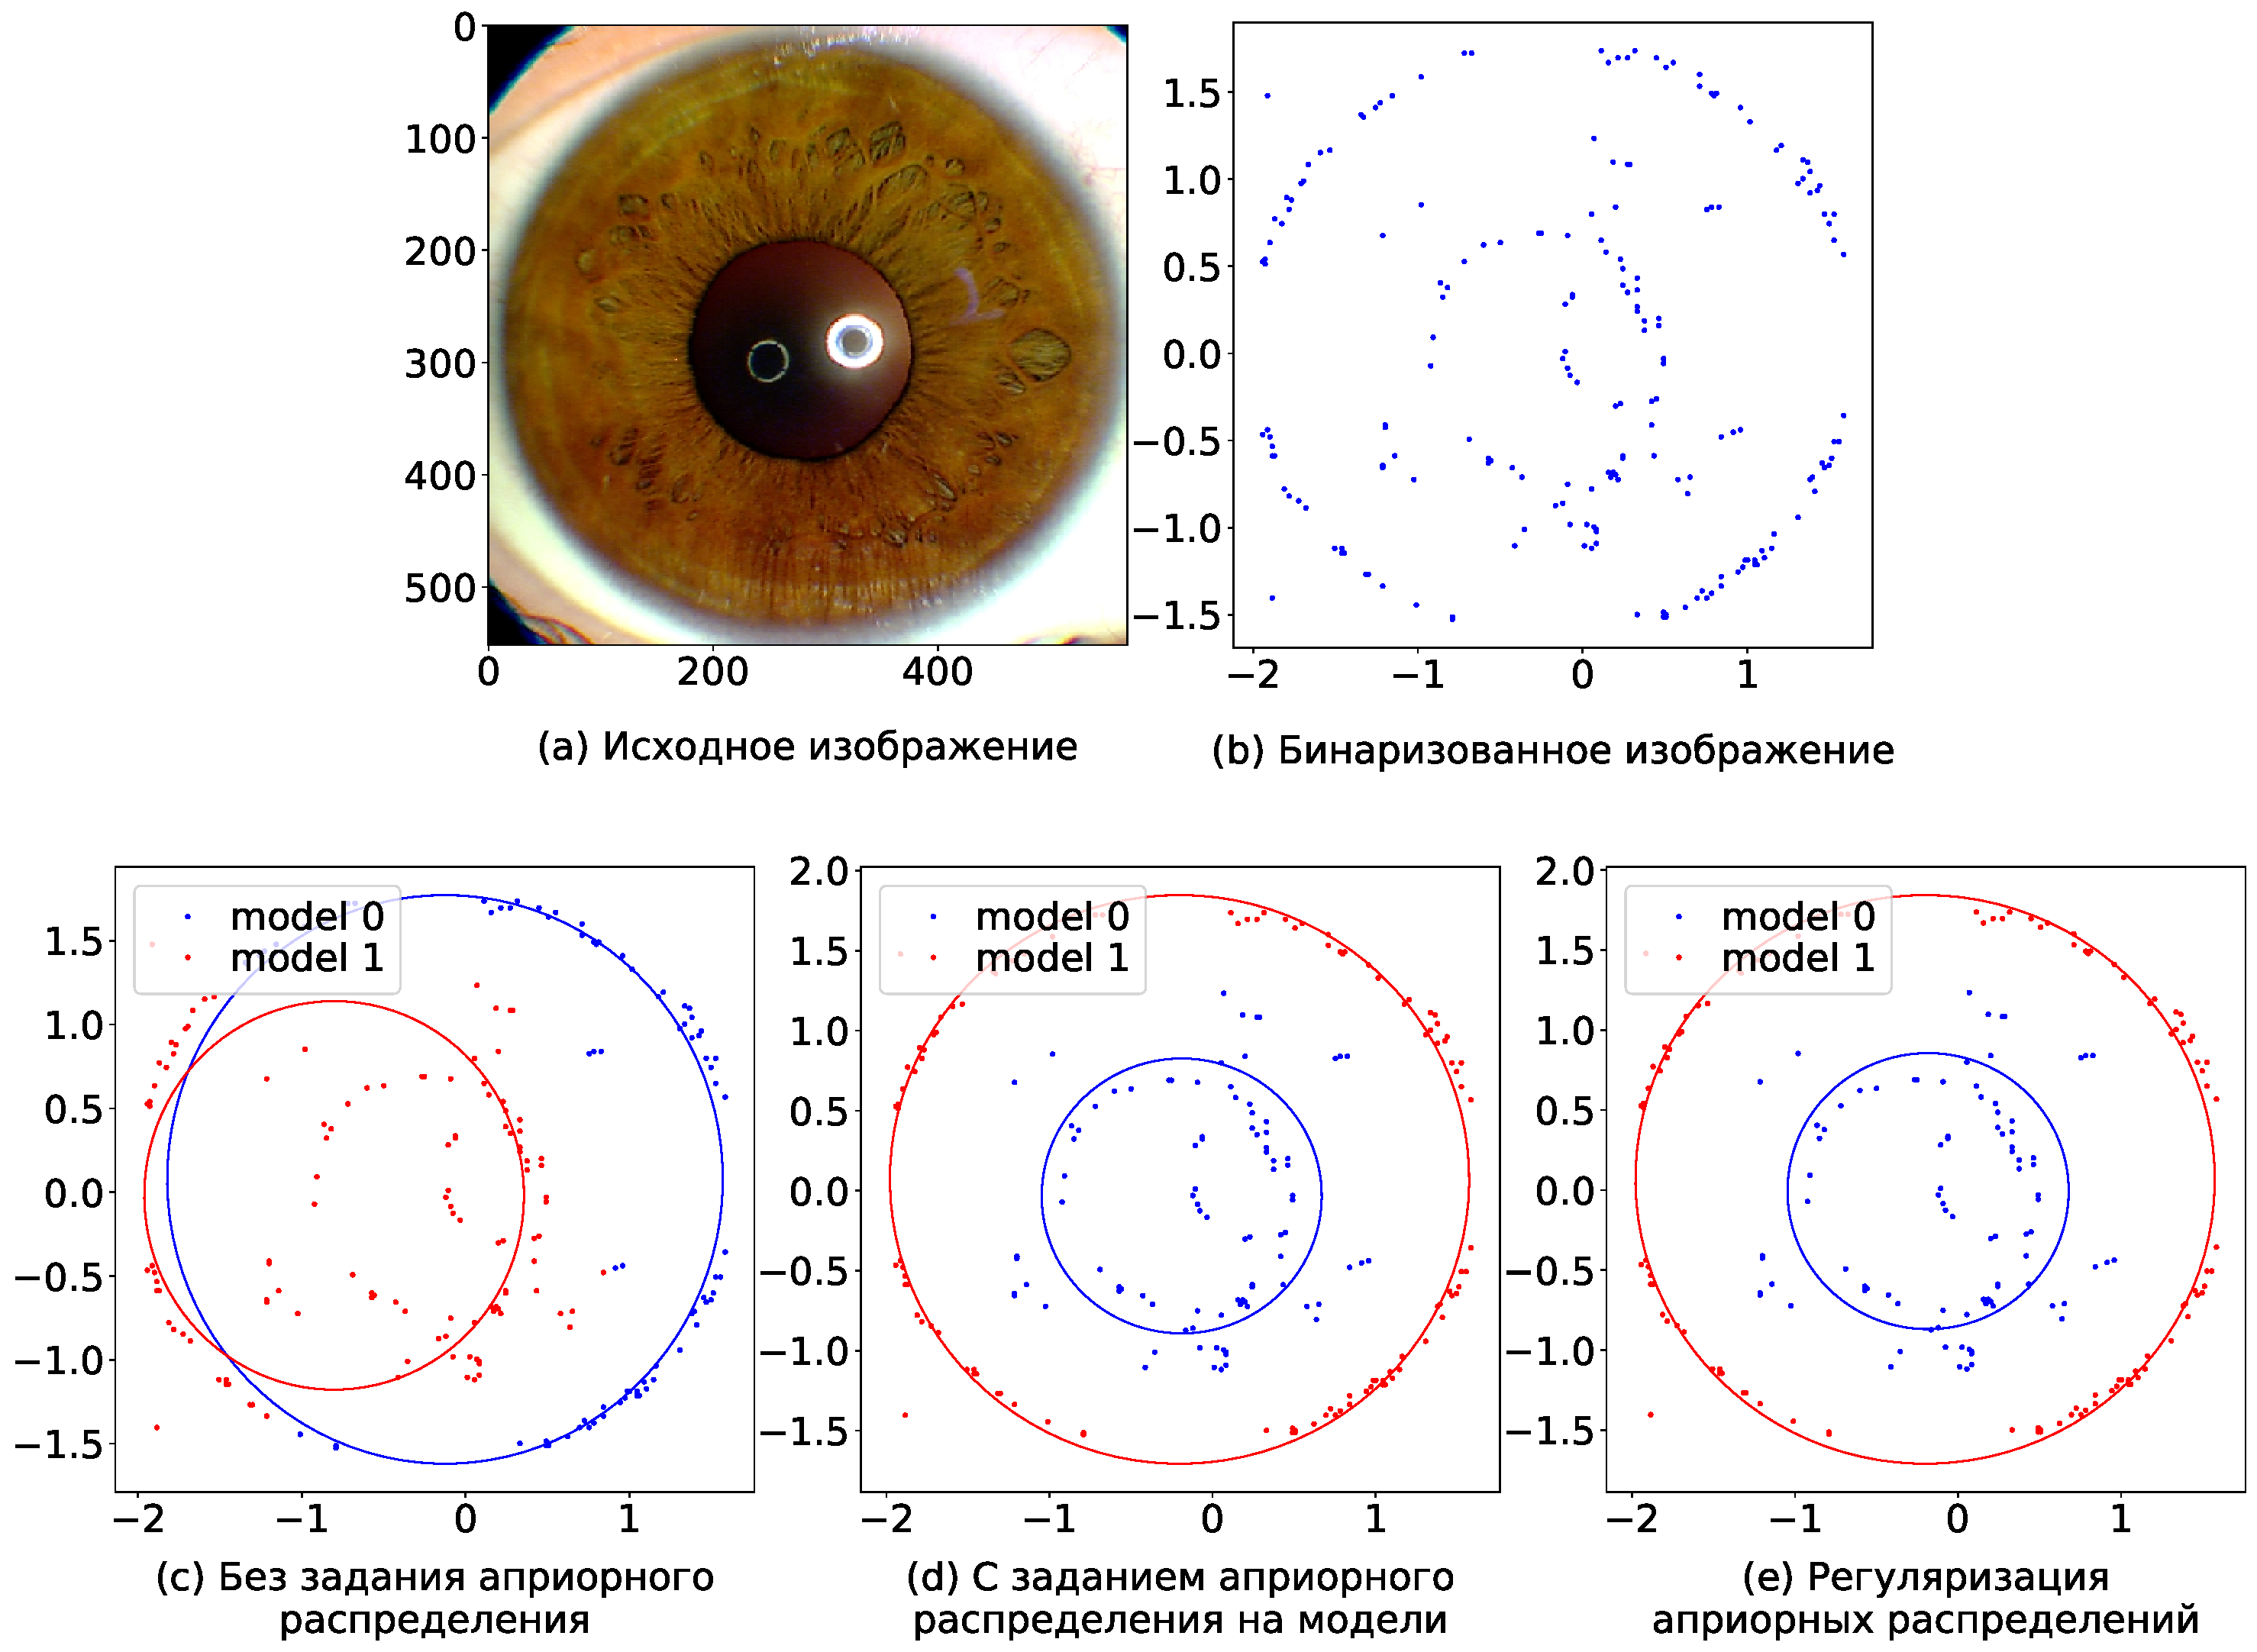
\includegraphics[height=0.9\textheight]{result/experiment_real_compare}
\end{center}

\end{frame}
%----------------------------------------------------------------------------------------------------------
\begin{frame}{Обучения на реальных данных}
\justifying
Регуляризация априорных распределений
\begin{center}
	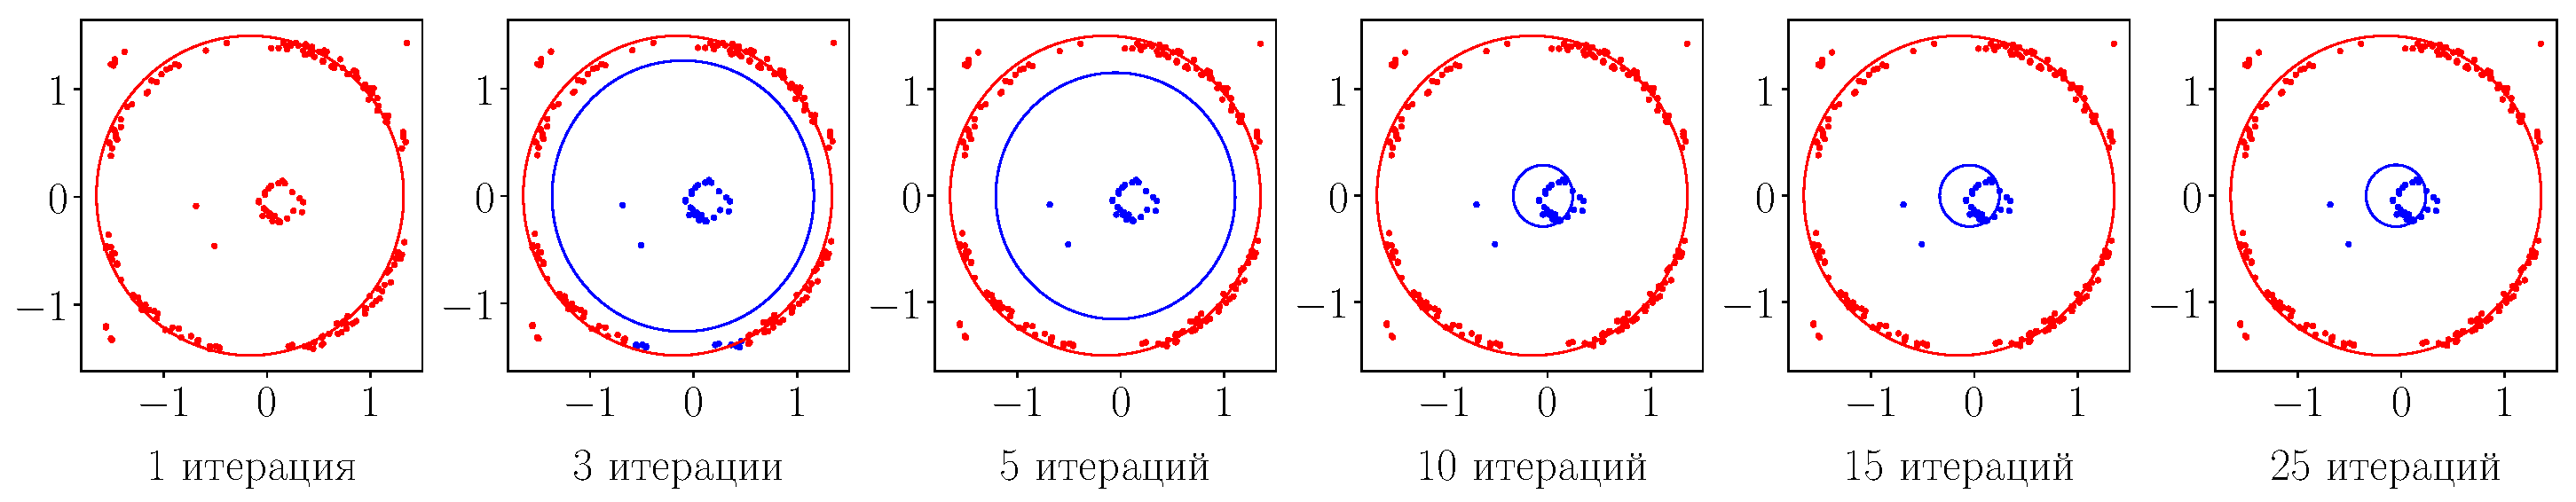
\includegraphics[width=0.95\textwidth]{result/experiment_real_regular}
\end{center}
С заданием априорного распределения на модели
\begin{center}
	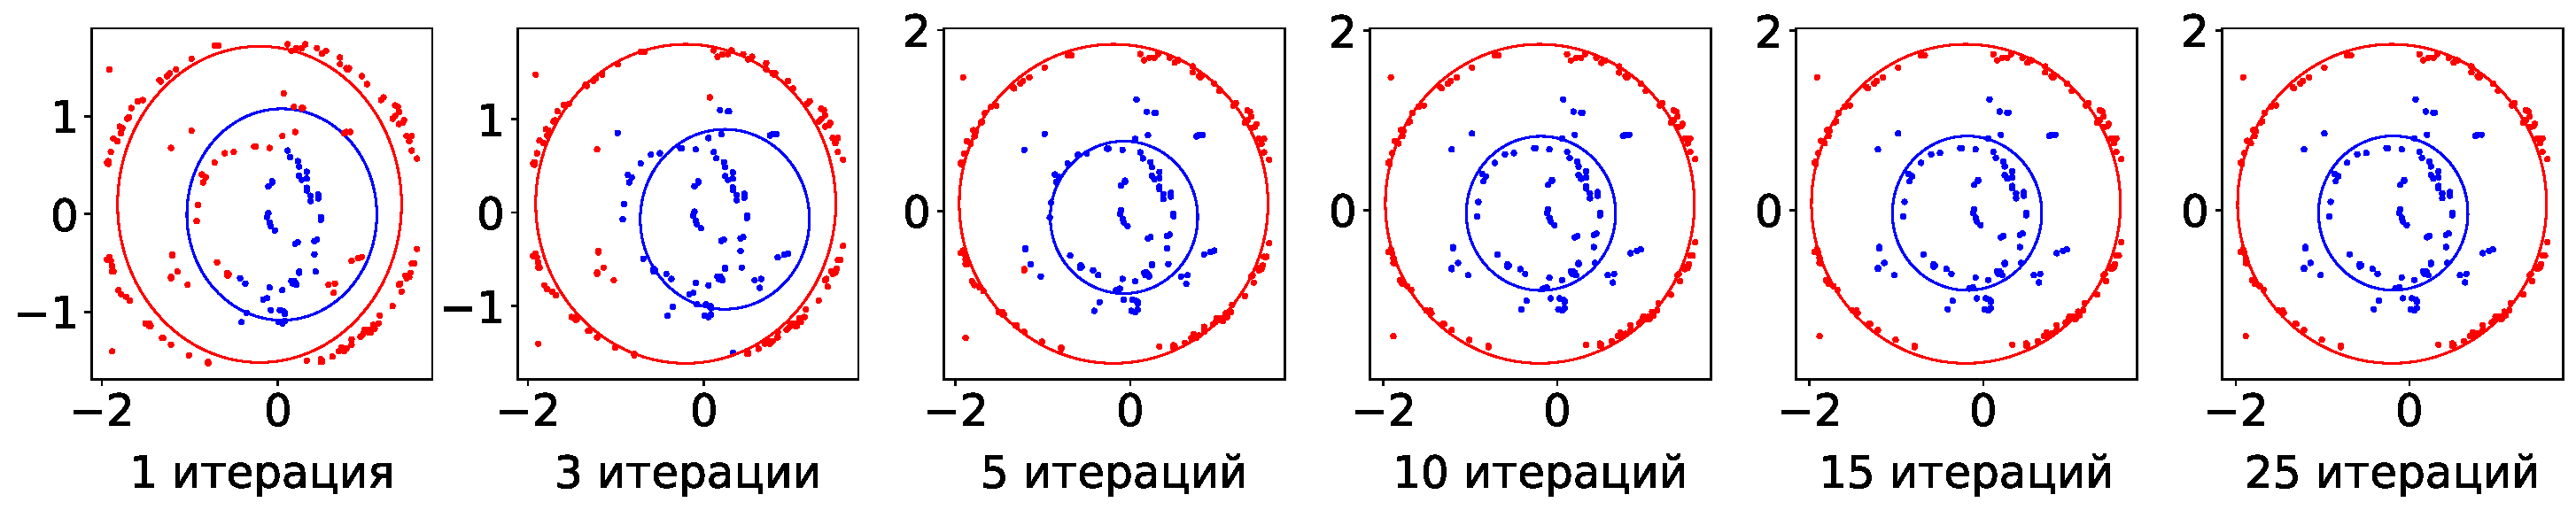
\includegraphics[width=0.95\textwidth]{result/experiment_real_prior}
\end{center}
Без задания априорного распределения
\begin{center}
	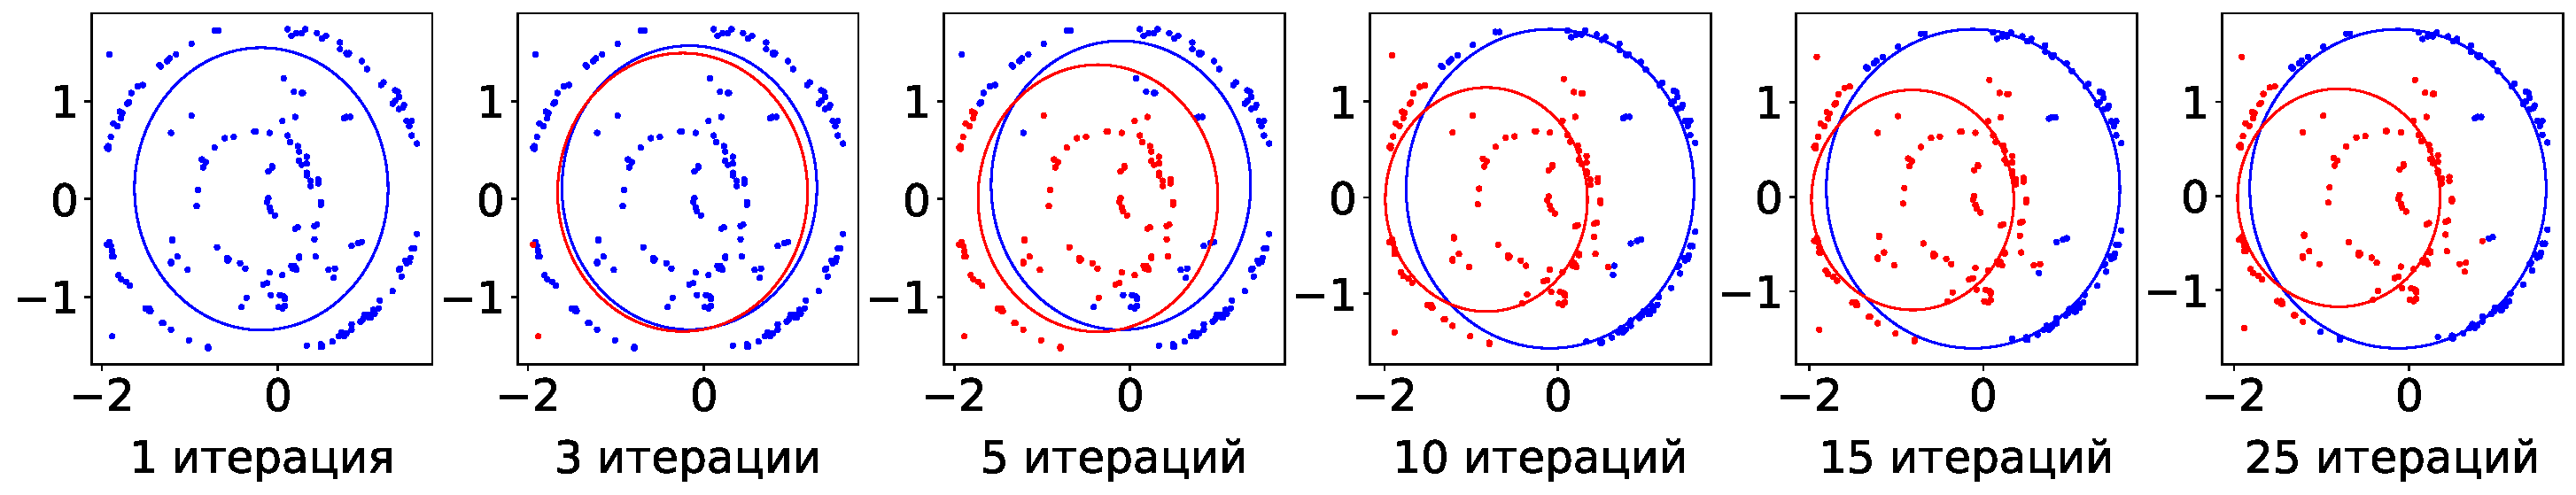
\includegraphics[width=0.95\textwidth]{result/experiment_real_not_prior}
\end{center}
\end{frame}
%----------------------------------------------------------------------------------------------------------
\begin{frame}{Вывод}
\justifying
Сделано:
	\begin{enumerate}
	\justifying
		\item Предложен метод поиска окружностей на бинарном изображении с различными априорными предположениями.
		\item Введено понятие регуляризации априорных распределений для улучшения качества мультимодели.
		\item В эксперименте показано, что задания регуляризации позволяет улучшить качество и устойчивость модели.
	\end{enumerate}

Планируется:
	\begin{enumerate}
	\justifying
		\item Улучшить мультимодель при помощи задания априорного распределения на шлюзовую функцию.
		\item Рассмотреть в качестве локальных моделей не только модели, которые описывают данные, а также модель, которая отвечает за шум в данных.
		\item Расширить класс локальных моделей с окружности до произвольной кривой второго порядка.
	\end{enumerate}	

\end{frame}
%----------------------------------------------------------------------------------------------------------





\end{document} 